\documentclass[10pt]{article}
\usepackage[margin=0.72in]{geometry}
\usepackage{amsmath,amssymb,amsthm,booktabs,graphicx,microtype,placeins,float}
\usepackage[font=small,skip=3pt]{caption}
\usepackage[hidelinks]{hyperref}
\setlength{\parindent}{0pt}
\setlength{\parskip}{3pt plus 1pt minus 1pt}
\setlength{\textfloatsep}{6pt plus 2pt minus 2pt}
\setlength{\intextsep}{6pt plus 2pt minus 2pt}
\newtheorem{theorem}{Theorem}
\newtheorem{proposition}[theorem]{Proposition}
\newcommand{\AON}{\mathrm{AON}}
\newcommand{\K}{K_{\mathcal L}}
\newcommand{\Khat}{\widehat K_{\mathcal L}}
\title{\vspace{-1.8em}\textbf{Prediction-Calibrated Refinement of Analytic Bounds}\\[-1pt]
\textbf{with an Application to Boolean Formula Complexity}}
\author{J. R. Landers}
\date{\vspace{-1.5em}}

\begin{document}
\maketitle
\vspace{-1.7em}

\begin{abstract}
Many hard optimization problems have a proved but loose analytic envelope
$L(x)\le Y(x)\le H(x)$ and exact solutions for small instances.  We formalize
a general refinement operator: center an interval at a prediction $\widehat
Y(x)$, calibrate its two error directions on held-out exact instances, and
intersect it with $[L(x),H(x)]$.  The refined interval is never wider than the
analytic envelope and preserves the calibration guarantee.  Depending on how
prediction error is controlled, this yields a statistical interval, an
exhaustively verified finite-domain bound, or a universal bound.  We apply
the framework to Boolean formula complexity.  If $K_{\mathcal L}(f)$ is the
fewest gates needed to compute $f$ over gate library $\mathcal L$, then
$\Khat(f)$ predicts that number from semantic features.  For NAND, NOR, and
AND/OR/NOT formulas, we calibrate around $\Khat(f)$ and intersect with a valid
Khrapchenko--construction envelope.
Over all 65,536 four-input functions, nominal 95\% intervals cover
96.3\%, 96.6\%, and 96.4\% of functions while removing 82.0\%, 79.2\%, and
71.5\% of the classical width.  Maximum-residual intervals cover the complete
finite universe and still remove 54.7\%, 57.1\%, and 47.9\%.  Feature
ablations show that the learned center improves materially over the envelope
midpoint.  We then freeze a dimension-compatible conditional-error protocol
and evaluate a newly enumerated five-input cost layer.  On 40 exact cost-11
functions per basis it covers 40/40 NAND, 40/40 NOR, and 37/40 AND/OR/NOT
functions while removing 94.7\%, 93.8\%, and 71.9\% of the applicable general
envelope.  We report statistical coverage, finite exhaustive certification,
and higher-dimensional transfer separately: prediction refines the useful
range, while the source of calibration determines the strength of the claim.
\end{abstract}

\section{Introduction}

Analytic bounds and learned predictions answer different questions.  A proof
may certify that an unknown quantity lies in a broad interval.  A predictor
may locate it accurately without supplying any certificate.  We ask how these
objects can be combined without weakening the proof or overstating the
prediction.

Our approach has four steps.  Theory first brackets the answer.  A model then
predicts where the answer lies inside that bracket.  Held-out examples measure
how far the predictions can miss.  Finally, we widen around the prediction by
those measured errors and intersect with the original theoretical bracket.
Thus theory supplies validity, while learning supplies localization.

The construction is deliberately simple: bracket, predict, calibrate, and
intersect.  Its value is that these four steps keep their meanings.  The
analytic envelope remains the guaranteed outer constraint; predictor quality
controls how much the interval can shrink; and the calibration protocol
determines whether the refined interval has statistical, finite-domain, or
universal validity.

Boolean formula complexity provides a demanding case study.  For a Boolean
function $f$, $K_{\mathcal L}(f)$ is the smallest number of gates in a tree
formula over library $\mathcal L$ that computes $f$.  Exact synthesis finds
$K$ only in small dimensions.  Classical theory gives dimension-independent
lower bounds and explicit constructive upper bounds, but often leaves a wide
gap.  We use exact small instances to learn and calibrate a location inside
that gap.  The prediction $\Khat(f)$ is not a formula and is not itself a
bound; it becomes useful only through calibrated error and intersection with
the analytic envelope.

Section 2 states the general refinement principle and separates its three
guarantee regimes.  Section 3 instantiates the envelope, predictor, and
calibration for Boolean formulas.  Sections 4 and 5 give a complete four-input
experiment and a frozen five-input stress test.  Sections 6 and 7 discuss the
route from statistical refinement to certified mathematical improvement.

\paragraph{Contributions.}  First, we state a general prediction-calibrated
operator for refining any valid analytic envelope and show that intersection
preserves the available error guarantee while never increasing width.  We
distinguish statistical, exhaustive finite-domain, and universal versions of
that guarantee.  Second, we instantiate the framework for exact Boolean
formula size using semantic lower bounds, constructive upper bounds, and a
learned center.  Over every four-input function the learned interval is much
narrower than both the analytic envelope and a calibrated midpoint baseline;
a maximum-error version covers the entire finite universe.  Finally, a frozen
five-input test preserves strong NAND/NOR shrinkage and exposes a specific AON
upper-tail failure.

Exact synthesis has long been used to classify small functions and benchmark
logic representations \cite{haaswijk2017,turan2015}.  Formula lower bounds,
including Khrapchenko's boundary method, pursue dimension-independent
obstructions \cite{khrapchenko1971,jukna2012}.  Conformal prediction supplies
finite-sample marginal coverage under exchangeability
\cite{vovk2005,lei2018}.  The present work connects these strands through a
reusable abstraction: theory supplies an outer envelope, prediction proposes
a center, and calibration supplies an explicitly qualified refinement.

\section{Calibrated refinement of analytic envelopes}

Let $x$ be an instance, $Y(x)$ an unknown real-valued target, and suppose
analysis supplies a valid envelope
\begin{equation}
 I_0(x)=[L(x),H(x)],\qquad L(x)\le Y(x)\le H(x).
 \label{eq:outer}
\end{equation}
Let $\widehat Y(x)$ be any point predictor.  Calibration supplies nonnegative
one-sided allowances $E^-(x)$ and $E^+(x)$, producing the prediction interval
$C(x)=[\widehat Y(x)-E^-(x),\widehat Y(x)+E^+(x)]$.  We define the refined
envelope by the intersection
\begin{equation}
 I_*(x)=I_0(x)\cap C(x)
 =\left[\max\{L,\widehat Y-E^-\},
         \min\{H,\widehat Y+E^+\}\right].
 \label{eq:refined}
\end{equation}
If the displayed lower endpoint exceeds the upper endpoint, $I_*(x)$ is the
empty set and its width is defined as zero.

\begin{proposition}[Envelope refinement]
\label{prop:refinement}
For every $x$, $I_*(x)\subseteq I_0(x)$ and therefore
$\operatorname{width}(I_*(x))\le\operatorname{width}(I_0(x))$.  Moreover, if
$I_0$ always contains $Y$ and $C$ contains $Y$ with probability at least
$1-\alpha$, then $I_*$ contains $Y$ with probability at least $1-\alpha$.
The same statement holds with ``probability'' replaced by validity on a fixed
finite domain or validity for every instance.
\end{proposition}
\emph{Proof.}  The width statement follows from intersection.  Because
$Y(x)\in I_0(x)$, the events $Y(x)\in I_*(x)$ and $Y(x)\in C(x)$ coincide.
The probabilistic and deterministic claims follow immediately. \qed

The proposition separates tightness from validity.  A more accurate predictor
usually needs smaller allowances and hence produces a narrower refinement.
The source of the allowances determines the claim.  Held-out quantiles give a
\emph{statistical} interval under their sampling assumption.  The largest
error over an exhaustively enumerated domain gives a \emph{finite-domain}
certificate.  A proved error bound that holds for every instance gives a
\emph{universal} refined bound.  The intersection operator is identical in
all three cases; only the status of $E^-$ and $E^+$ changes.

For exact calibration labels, define one-sided residuals
\begin{equation}
 R^-(x)=(\widehat Y(x)-Y(x))_+,
 \qquad R^+(x)=(Y(x)-\widehat Y(x))_+,
 \label{eq:residuals}
\end{equation}
where $(z)_+=\max\{z,0\}$.  In grouped split conformal calibration, instances
with the same observable profile form one class, and the class score is its
largest member residual.  With $m$ calibration classes and total error rate
$\alpha$, $E^-$ and $E^+$ are the
$\lceil(m+1)(1-\alpha/2)\rceil$-th ordered class scores, using an unbounded
allowance if that rank exceeds $m$.  If calibration and test classes are
exchangeable---their ordering carries no information about their errors---a
union bound over the two tails gives coverage at least $1-\alpha$ for every
member of the test class \cite{vovk2005,lei2018}.

\section{Boolean formula complexity instantiation}

\subsection{Exact cost and analytic envelope}

For $f:\{0,1\}^n\to\{0,1\}$ and gate library $\mathcal L$, define
\[
 K_{\mathcal L}(f)=\min\{|e|:\operatorname{eval}_{\mathcal L}(e)=f\}.
\]
Here $e$ ranges over tree formulas, $|e|$ counts gates, variables are free
leaves, fanout is one, and constants are not free.  We study NAND, NOR, and
$\AON=\{\text{AND},\text{OR},\text{NOT}\}$.

Write $Z=f^{-1}(0)$ and $O=f^{-1}(1)$ for the zero and one inputs.  Two inputs
are neighbors when they differ in one bit, and $E_{01}$ is the set of
neighboring pairs on which $f$ changes value.  The Khrapchenko quantity is
\begin{equation}
 B(f)=\frac{|E_{01}|^2}{|Z||O|}=\bar s_0(f)\bar s_1(f),
 \label{eq:khrapchenko}
\end{equation}
where $\bar s_0$ and $\bar s_1$ are the average numbers of value-changing
neighbors seen from $Z$ and $O$; set $B=0$ for constants.  Khrapchenko's
theorem lower-bounds formula leaves by $B$.  Moving NOT gates to the inputs
does not change the leaf count, so all three libraries satisfy
\begin{equation}
 B(f)\le K_{\mathcal L}(f)+1.
 \label{eq:lower}
\end{equation}

Let $U(f)$ be the smallest number of leaves in a deterministic decision tree
for $f$.  Recursively converting the tree to a formula gives
\begin{align}
 K_{\mathrm{NAND}}(f)+1,\ K_{\mathrm{NOR}}(f)+1
   &\le 6+9(U(f)-1),\nonumber\\
 K_{\AON}(f)+1&\le 3+6(U(f)-1).
 \label{eq:general-upper}
\end{align}
For AON, $Q_{\min}(f)$ is the smallest gate count among the prime disjunctive
and conjunctive normal-form constructions we enumerate, including variants
with one outer NOT.  It is a valid constructive upper bound.  Finding the
least such cover is weighted set cover \cite{allender2006}, and every returned
cover is an explicit formula witness.

Exhaustive synthesis tightens the coefficients on the four-input universe:
\begin{align}
 B(f)&\le K_{\mathrm{NAND/NOR}}(f)+1
       \le 6+\tfrac94(U(f)-1),\nonumber\\
 B(f)&\le K_{\AON}(f)+1
       \le\min\{3+\tfrac{13}{9}(U(f)-1),Q_{\min}(f)\}.
 \label{eq:four-upper}
\end{align}
These coefficients are finite-domain facts, not arbitrary-dimension claims.

\subsection{Learned center and calibration}

Set $Y_{\mathcal L}(f)=K_{\mathcal L}(f)+1$ because the lower bound naturally
counts leaves.  Let $[L_{\mathcal L}(f),H_{\mathcal L}(f)]$ be the envelope
from \eqref{eq:lower} and either \eqref{eq:general-upper} or
\eqref{eq:four-upper}.  We predict the normalized location
\begin{equation}
 \rho_{\mathcal L}(f)=\frac{Y_{\mathcal L}(f)-L_{\mathcal L}(f)}
 {H_{\mathcal L}(f)-L_{\mathcal L}(f)},
 \qquad
 \widehat Y=L+\widehat\rho(\Phi(f))(H-L),
 \qquad \Khat=\widehat Y-1.
 \label{eq:center}
\end{equation}
If $L=H$, the answer is known and we set $\rho=1/2$.  Thus $\Khat(f)$ is the
predicted minimum gate count, not the cost of a constructed formula and not a
proved bound.

The 16-entry feature vector $\Phi(f)$ contains $(B,U)$, four summaries of
explicit constructions, counts of monomials by degree in the algebraic normal
form (the unique polynomial over the two-element field), and counts of
negative Fourier--Walsh coefficients by degree.  A gradient-boosted tree
predicts $\rho$, clipped to $[0,1]$.  For transfer beyond four inputs, degrees
are grouped into bins $0,1,2,3,$ and $4+$.

Functions with the same $\Phi$ form one calibration class.  We apply the
grouped residual construction from Section 2, using the largest error in each
class.  Five rotating train/calibrate/test splits provide the reported 95\%
coverage.  Separately, setting $E^\pm$ to the largest cross-fitted residual on
all 65,536 four-input functions gives an exhaustively verified finite-domain
instance of Proposition~\ref{prop:refinement}.  It makes no claim about
dimension five.

\FloatBarrier
\section{Complete four-input experiment}

We synthesize exact minima for every four-input function in all three bases.
Among the 65,536 truth tables there are 3,952 distinct feature vectors
$\Phi$.  We divide these profile classes into five folds, keeping functions
with identical features together.  In each rotation, three folds fit the
model, one sets the error allowances, and one tests the resulting intervals.
The stated 95\% target assigns 2.5\% error to each tail.  ``Coverage'' is the
fraction of held-out exact values inside the interval.  ``Shrinkage'' is the
fraction of the original interval width removed.  Candidate counts round the
endpoints inward and count the remaining integer values that $K+1$ could take.

\begin{table}[H]
\centering\small
\begin{tabular}{lrrrrr}
\toprule
basis & function cov. & profile cov. & shrink & candidates & full shrink\\
\midrule
NAND & .963 & .951 & .820 & $18.35\to3.23$ & .547\\
NOR  & .966 & .953 & .792 & $18.35\to3.74$ & .571\\
AON  & .964 & .952 & .715 & $9.15\to2.48$  & .479\\
\bottomrule
\end{tabular}
\caption{Four-input results. Coverage and shrinkage use 95\% profile-grouped
calibration. ``Candidates'' is the mean number of possible integer values for
$K+1$, before and after calibration around $\widehat K$. ``Full shrink'' uses
the largest observed errors and covers the entire four-input universe.}
\label{tab:n4}
\end{table}

Table~\ref{tab:n4} gives the central result.  Calibration around $\widehat K$
reduces roughly 9--18 possible gate counts to 2--4, while held-out coverage is
near the stated 95\% level.  Function coverage is slightly higher than profile
coverage because every profile is scored by its worst member.  If we instead
use the largest cross-fitted error anywhere in the complete data set, all
65,536 functions are covered and the intervals still lose roughly half their
original width.

\paragraph{Does learning matter?}
A calibrated interval around any center can shrink a loose outer bound.  We
therefore repeat the complete protocol with a fixed midpoint and with feature
families removed.  Table~\ref{tab:ablation} reports the fraction of integral
candidates removed at comparable realized coverage.

\begin{table}[H]
\centering\small
\begin{tabular}{lrrr}
\toprule
center/features & NAND & NOR & AON\\
\midrule
fixed midpoint       & .612 & .612 & .547\\
theory features $B,U$ & .643 & .639 & .615\\
construction features & .715 & .717 & .582\\
ANF + Fourier features & .737 & .697 & .619\\
all non-endpoint features & .799 & .777 & .650\\
all 16 features       & \textbf{.820} & \textbf{.792} & \textbf{.717}\\
\bottomrule
\end{tabular}
\caption{Mean reduction in feasible integer candidates at 95\% coverage.
Each non-midpoint row trains a separate predictor using only the named feature
family; ``all non-endpoint'' omits $B$ and $U$. The 16-feature model improves
materially over the fixed center of the theoretical interval.}
\label{tab:ablation}
\end{table}

The full model leaves 3.23, 3.74, and 2.48 candidates on average, compared
with 6.96, 6.97, and 4.03 for the midpoint.  Thus the improvement is not merely
a consequence of calibrating any center inside a broad interval.  Explicit
construction features and the ANF/Fourier features provide information beyond
the two theoretical endpoints $(B,U)$.

\begin{figure}[H]
\centering
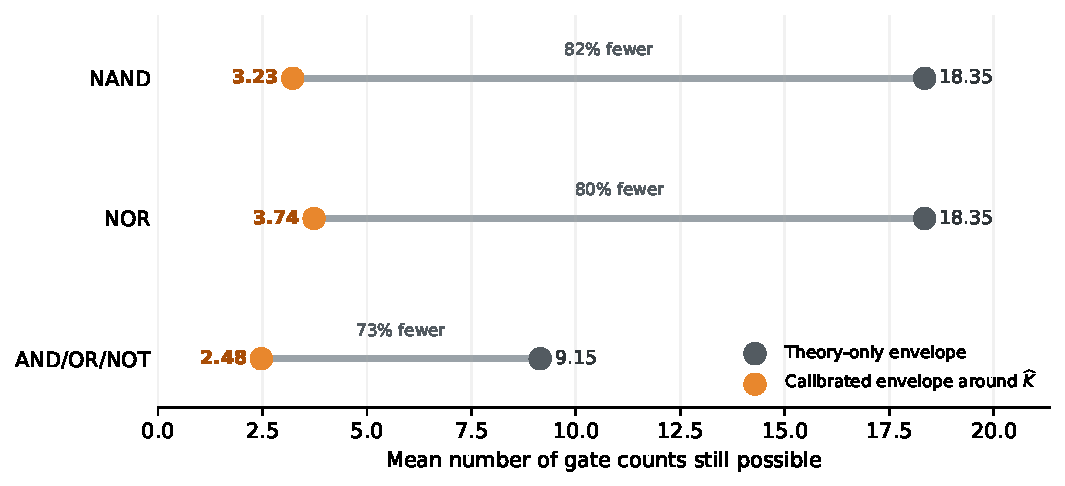
\includegraphics[width=0.82\textwidth]{../../experiments/four_bit/figures/learned_envelope_shrinkage.pdf}
\caption{Mean number of integer gate counts allowed by theory alone and after
95\% calibration around $\widehat K$.  The percentage is the reduction in
remaining candidates.  Intersecting with the theory-only interval preserves
all established lower and upper bounds.}
\label{fig:shrink}
\end{figure}

\FloatBarrier
\section{Frozen five-input stress test}

Exhaustively synthesizing all $2^{32}$ five-input truth tables is impractical
with the four-input method.  Instead, sparse dynamic programming enumerates
every function that can first be computed using at most 11 gates.  ``First
reached at cost 11'' certifies that no formula with fewer gates computes that
function.  This gives exact cost
for 4,434,723 NAND functions, the same number of NOR functions, and 15,631,538
AON functions.  From each exact-cost layer we select at most 40 functions by
a fixed seed.  The resulting distribution is balanced by formula cost and is
not uniform over truth tables.

We refit the predictor on four-input data, now using the general theoretical
endpoints \eqref{eq:general-upper} rather than the four-input-only coefficients
\eqref{eq:four-upper}.  The AON upper
endpoint still uses $Q_{\min}$ when smaller.  Initial checks showed that error
size changes with both input dimension and formula cost, so a single fixed
error allowance would be inappropriate.  Before enumerating cost 11, we
therefore freeze two models that predict lower- and upper-side error size from
$\widehat Y$, the original interval width, $(B,U)$, construction features,
and ANF/Fourier counts.  Samples through cost 9 fit these error models.  Cost
10 sets one final maximum-residual correction.  Cost 11 is then evaluated
once, without revising the method.
The frozen protocol and its SHA-256 digest are checked in with the
experimental artifacts.

\begin{table}[H]
\centering\small
\begin{tabular}{lrrrrrr}
\toprule
basis & train & cal. & test & covered & mean width & shrink\\
\midrule
NAND & 340 & 40 & 40 & 40/40 & 4.38 & .947\\
NOR  & 340 & 40 & 40 & 40/40 & 5.09 & .938\\
AON  & 350 & 40 & 40 & 37/40 & 4.06 & .719\\
\bottomrule
\end{tabular}
\caption{Prospective cost-11 conditional-envelope results.  The corresponding
mean classical widths are 83.08, 81.25, and 14.57.}
\label{tab:n5}
\end{table}

Table~\ref{tab:n5} asks whether the same story survives a harder, untouched
test: does $\widehat K$ still locate exact size, and do the previously
calibrated errors remain large enough?  This is evidence of transfer, not a
coverage theorem.  Costs 10 and 11 are different distributions, and a sample
of 40 functions per library has substantial uncertainty.  NAND and NOR retain
more than 93\% shrinkage with no sampled miss.  AON starts from a much tighter
theoretical interval, but three exact sizes fall above the learned upper
endpoint.  Those failures suggest that the current features miss some
recursive or factorized AON constructions.

\FloatBarrier
\section{Scope and next tests}

Proposition~\ref{prop:refinement} is an elementary intersection principle,
not a new complexity lower bound.  Its general value is organizational: it
identifies exactly which component supplies outer validity, localization, and
error control.  The framework can be used whenever a target has a valid
analytic envelope and representative exact or certified calibration labels.
It is useful only to the extent that the predictor reduces residual error and
the chosen calibration population matches the intended test population.

The complete four-input result is the strongest claim: every target size is
exact, functions with identical features stay together, and the
maximum-error interval is verified over the entire finite universe.  The 95\%
interval is narrower but makes the exchangeability assumption stated in
Section 2.  In neither case does $\widehat K$ become a theorem by itself.

The five-input experiment tests a harder proposition---whether the center and
its error geometry transfer across dimension.  Its layer-balanced sampling is
useful for controlled extrapolation but differs sharply from a random Boolean
function, a random semantic profile, or a benchmark distribution.  Larger
tests must freeze both the sampling measure and the conditional calibration
before exact synthesis.  In particular, the next untouched experiment should
oversample the AON upper tail and record prime-cover slack, factorability, and
restriction decompositions without revising the cost-11 result.

There are two routes from a useful prediction to a proof.  For an upper bound,
a predictor can choose among decision trees, covers, restrictions, and
factorizations; once it outputs an actual formula, its gate count is certified
regardless of prediction error.  A new lower bound is harder: it requires
either exhaustive finite verification or a new inequality that holds for all
formulas.  This asymmetry makes prediction-guided construction the clearest
next route to a dimension-general certified improvement.

\section{Conclusion}

A valid analytic envelope can be refined without confusing prediction with
proof.  Intersecting it with a calibrated interval around $\widehat Y$ never
widens the envelope and inherits whatever statistical, finite-domain, or
universal error guarantee supports the calibrated interval.  Predictor
quality determines tightness; calibration determines the strength of the
claim.

Boolean formula complexity demonstrates the distinction.  $\widehat K$
locates exact size inside a theory-supplied range.  Over all four-input
functions, calibration removes roughly three quarters of the uncertainty at
95\% coverage and roughly half under a 100\% finite certificate.  A frozen
five-input experiment preserves strong NAND/NOR shrinkage and reveals a
specific AON upper-tail weakness.  Thus the general method provides a clean
bridge from analytic bounds to useful predictions, while leaving the source
and limits of validity visible.

\paragraph{Reproducibility.}
All exact targets, folds, predictions, calibration tables, protocol hashes,
figures, and scripts are included in the accompanying repository.  Automated
tests verify the classical inequalities, finite learned intervals, generic
feature implementation, exact sparse layer separation, and held-out cost
boundaries.

\begingroup
\footnotesize
\setlength{\parskip}{0pt}
\begin{thebibliography}{9}
\setlength{\itemsep}{0pt}
\bibitem{khrapchenko1971}
V.~M. Khrapchenko, ``Method of determining lower bounds for the complexity of
$\Pi$-schemes,'' \emph{Math. Notes}, 10(1):474--479, 1971.
\bibitem{jukna2012}
S. Jukna, \emph{Boolean Function Complexity: Advances and Frontiers}.
Springer, 2012.
\bibitem{allender2006}
E. Allender, L. Hellerstein, P. McCabe, T. Pitassi, and M. Saks,
``Minimizing DNF formulas and $\mathrm{AC}^0$ circuits given a truth table,''
in \emph{Proc. IEEE CCC}, 2006.
\bibitem{haaswijk2017}
W. Haaswijk, E. Testa, M. Soeken, and G. De Micheli,
``Classifying functions with exact synthesis,'' in \emph{Proc. IEEE ISMVL},
2017.
\bibitem{turan2015}
M. S. Turan and R. C. Peralta, ``The multiplicative complexity of Boolean
functions on four and five variables,'' in \emph{LIGHTSEC}, 2015.
\bibitem{vovk2005}
V. Vovk, A. Gammerman, and G. Shafer,
\emph{Algorithmic Learning in a Random World}. Springer, 2005.
\bibitem{lei2018}
J. Lei, M. G'Sell, A. Rinaldo, R. Tibshirani, and L. Wasserman,
``Distribution-free predictive inference for regression,''
\emph{J. Amer. Statist. Assoc.}, 113(523):1094--1111, 2018.
\end{thebibliography}
\endgroup

\end{document}
